% !Mode:: "TeX:UTF-8:Main"
% gif command (hope it still works ...)
% magick -density 160 -delay 35 -loop 0 XXXX.pdf XXXX.gif
\PassOptionsToPackage{svgnames}{xcolor}
\documentclass{beamer}
\usepackage[T1]{fontenc} % or fontspec if lualatex is wanted ...
\setbeamertemplate{navigation symbols}{}
\usepackage{tikzducks,tikzlings}
\usepackage{bearwear}
\definecolor{mask}{RGB}{171,201,177}
\definecolor{swissred}{RGB}{216,30,5}
\tikzset{swisscross/.pic={
\begin{scope}[y=0.80pt, x=0.80pt,
yscale=-1,yshift=-240]
%\path[fill=swissred,rounded corners=0.0000cm] (0.0000,0.0000) rectangle
%  (300.0000,300.0000);
\path[fill=swissred,rounded corners=0.0000cm] (50.0000,120.0000) rectangle
  (250.0000,180.0000);
\path[fill=swissred,rounded corners=0.0000cm] (120.0000,50.0000) rectangle
  (180.0000,250.0000);
\end{scope}
}}
\begin{document}%
%Anteater . . . . . . . . . . . . . . . . . . . . . . . . . . . . . . . . . . . . . . . . . . . . . . . . . . 4
%done Bear . . . . . . . . . . . . . . . . . . . . . . . . . . . . . . . . . . . . . . . . . . . . . . . . . . . . . 5
%done Bee . . . . . . . . . . . . . . . . . . . . . . . . . . . . . . . . . . . . . . . . . . . . . . . . . . . . . 7
%done Cat . . . . . . . . . . . . . . . . . . . . . . . . . . . . . . . . . . . . . . . . . . . . . . . . . . . . . 9
%Coati . . . . . . . . . . . . . . . . . . . . . . . . . . . . . . . . . . . . . . . . . . . . . . . . . . . . 12
%done Hippo . . . . . . . . . . . . . . . . . . . . . . . . . . . . . . . . . . . . . . . . . . . . . . . . . . . . 14
%done Koala . . . . . . . . . . . . . . . . . . . . . . . . . . . . . . . . . . . . . . . . . . . . . . . . . . . . 16
%Marmot . . . . . . . . . . . . . . . . . . . . . . . . . . . . . . . . . . . . . . . . . . . . . . . . . . . 18
%Mole . . . . . . . . . . . . . . . . . . . . . . . . . . . . . . . . . . . . . . . . . . . . . . . . . . . . 20
%Mouse . . . . . . . . . . . . . . . . . . . . . . . . . . . . . . . . . . . . . . . . . . . . . . . . . . . 22
%Owl . . . . . . . . . . . . . . . . . . . . . . . . . . . . . . . . . . . . . . . . . . . . . . . . . . . . . 24
%Panda . . . . . . . . . . . . . . . . . . . . . . . . . . . . . . . . . . . . . . . . . . . . . . . . . . . . 26
%Penguin . . . . . . . . . . . . . . . . . . . . . . . . . . . . . . . . . . . . . . . . . . . . . . . . . . 27
%Pig . . . . . . . . . . . . . . . . . . . . . . . . . . . . . . . . . . . . . . . . . . . . . . . . . . . . . . 29
%done Rhino . . . . . . . . . . . . . . . . . . . . . . . . . . . . . . . . . . . . . . . . . . . . . . . . . . . . 30
%Sloth . . . . . . . . . . . . . . . . . . . . . . . . . . . . . . . . . . . . . . . . . . . . . . . . . . . . 32
%Squirrel . . . . . . . . . . . . . . . . . . . . . . . . . . . . . . . . . . . . . . . . . . . . . . . . . . . 34
%Snowman . . . . . . . . . . . . . . . . . . . . . . . . . . . . . . . . . . . . . . . . . . . . . . . . . 35
\makeatletter
\begin{frame}
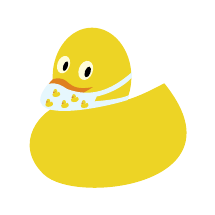
\begin{tikzpicture}
	\duck[]

  \begin{pgfinterruptboundingbox}
    \fill[cyan!10!white]  (1.4051,1.5586) .. controls (1.1370,1.3225) and (0.8775,1.2365) .. (0.5844,1.3462) .. controls (0.5190,1.3848) and (0.4601,1.4391) .. (0.3414,1.4100) .. controls (-0.1044,0.8610) and (1.0760,1.1140) .. (1.3547,1.2073) -- (1.3698,1.2679) .. controls (1.2783,1.2261) and (1.1035,1.2035) .. (0.9324,1.1895) -- (0.9600,1.2509) .. controls (1.1068,1.2809) and (1.2985,1.3700) .. (1.4071,1.4930) -- cycle;
  \end{pgfinterruptboundingbox}

  \duck[scale=0.05, shift={(6,22.3)}]
  \duck[scale=0.05, shift={(7.8,24.8)}]
  \duck[scale=0.05, shift={(10,22)}]
  \duck[scale=0.05, shift={(12.5,23.5)}]
  \duck[scale=0.05, shift={(15,22)}]

\end{tikzpicture}	
\end{frame}
\end{document}

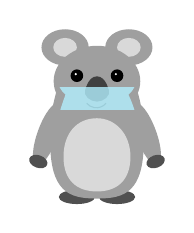
\begin{tikzpicture}
\koala
\begin{scope}
		\clip   (-0.1,2.1) to[out=180,in=140,looseness=1.2] (-0.4,1.5) to[out=-110,in=180,looseness=1.2] (-0.1,0.15) to[out=00,in=-65,looseness=1.2] (0.4,1.5) to[out=40,in=0,looseness=1.2] cycle;

       \fill[blue!20!cyan!30!white,opacity=0.8] (-3,1.3) rectangle (3,1.6);
\end{scope}
\end{tikzpicture}


%\begin{tikzpicture}
%\anteater
%%\begin{scope}
%%		\clip (0, 1.55) ellipse[x radius=0.42, y radius=0.2];
%%       \fill[mask!80!red] (-3,1.45) rectangle (3,1.65);
%%\end{scope}
%\end{tikzpicture}

%\begin{tikzpicture}
%\coati
%\begin{scope}
%		\clip   (0,2.1) to[out=180,in=140,looseness=1.2] (-0.3,1.5) to[out=-110,in=180,looseness=1.2] (0,0.15) to[out=00,in=-65,looseness=1.2] (0.3,1.5) to[out=40,in=0,looseness=1.2] cycle;
%
%       \fill[blue!20!cyan!30!white,opacity=0.8] (-3,1.5) rectangle (3,1.7);
%\end{scope}
%\end{tikzpicture}

\end{frame}
\end{document}

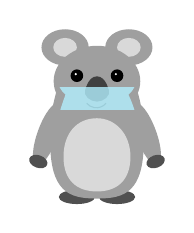
\begin{tikzpicture}
\koala
\begin{scope}
		\clip   (-0.1,2.1) to[out=180,in=140,looseness=1.2] (-0.4,1.5) to[out=-110,in=180,looseness=1.2] (-0.1,0.15) to[out=00,in=-65,looseness=1.2] (0.4,1.5) to[out=40,in=0,looseness=1.2] cycle;

       \fill[blue!20!cyan!30!white,opacity=0.8] (-3,1.3) rectangle (3,1.6);
\end{scope}
\end{tikzpicture}

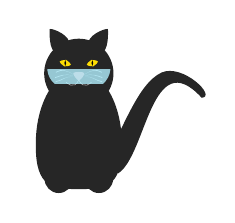
\begin{tikzpicture}
\cat
\begin{scope}
		\clip   (0,2.1) to[out=180,in=140,looseness=1.2] (-0.3,1.5) to[out=-110,in=180,looseness=1.2] (0,0.15) to[out=00,in=-65,looseness=1.2] (0.3,1.5) to[out=40,in=0,looseness=1.2] cycle;

       \fill[blue!20!cyan!30!white,opacity=0.8] (-3,1.5) rectangle (3,1.7);
\end{scope}
\end{tikzpicture}

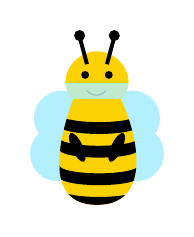
\begin{tikzpicture}
\bee
\begin{scope}
		\clip   (0,2.1) to[out=180,in=140,looseness=1.2] (-0.3,1.5) to[out=-110,in=180,looseness=1.2] (0,0.15) to[out=00,in=-65,looseness=1.2] (0.3,1.5) to[out=40,in=0,looseness=1.2] cycle;

       \fill[blue!20!cyan!30!white,opacity=0.8] (-3,1.5) rectangle (3,1.7);
\end{scope}
\end{tikzpicture}


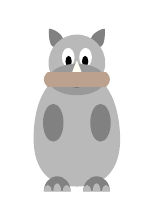
\begin{tikzpicture}
\rhino
\begin{scope}
		\clip (0, 1.55) ellipse[x radius=0.42, y radius=0.2];
       \fill[mask!80!red] (-3,1.45) rectangle (3,1.65);
\end{scope}
\end{tikzpicture}


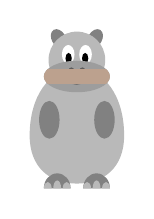
\begin{tikzpicture}
\hippo
\begin{scope}
		\clip (0, 1.55) ellipse[x radius=0.42, y radius=0.2];
       \fill[mask!80!red] (-3,1.45) rectangle (3,1.65);
\end{scope}
\end{tikzpicture}


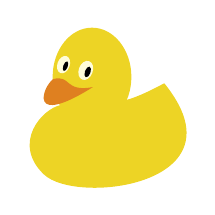
\begin{tikzpicture}
\duck
\end{tikzpicture}

\begin{tikzpicture}\bear\bearwear[shirt=white,t-shirt,body deco={\path (beartummy)--++(0.1,-0.1) pic[scale=0.04]{swisscross};}]
\begin{scope}
		\clip (0, 1.55) circle (0.5);
       \fill[mask!80!black] (-3,1.25) rectangle (3,1.6);
\end{scope}
\draw[\bear@body!70!white!80!red] (0, 1.5) ellipse (0.15 and 0.08);
\draw[\bear@body!30!black,line width=0.4pt] (0.145, 1.38) arc [start angle=-20, end angle=-160, radius=0.16];
%
%\path (0,0) pic{swisscross};
\end{tikzpicture}

